\begin{frame}
\frametitle{Problem and Motivation}
\begin{Example}
\pause
\begin{figure}[h]
	\centering
		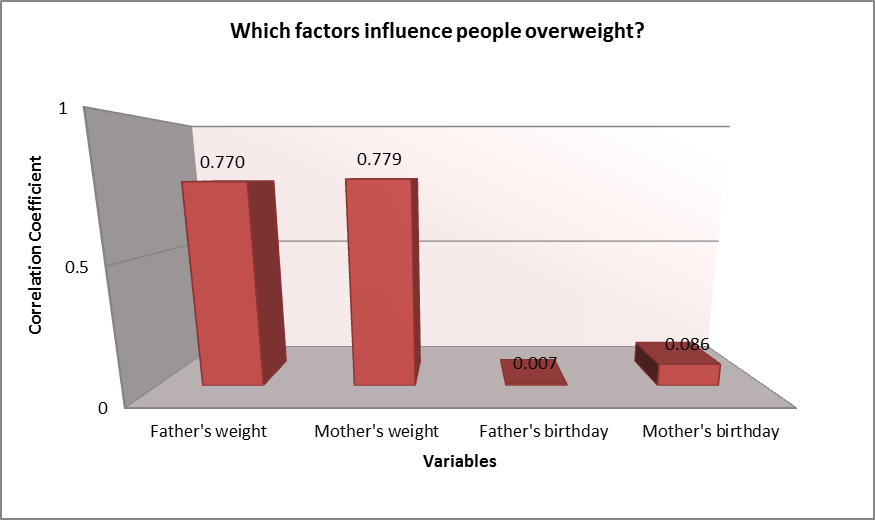
\includegraphics[width=0.8\textwidth]{../Images/example01}       
	\caption{Correlation analysis of input variables.}
	\label{fig:example01}
\end{figure}
\end{Example}
\end{frame}

\begin{frame}
\frametitle{Problem and Motivation}
\begin{Example}
\begin{figure}[h]
	\centering
		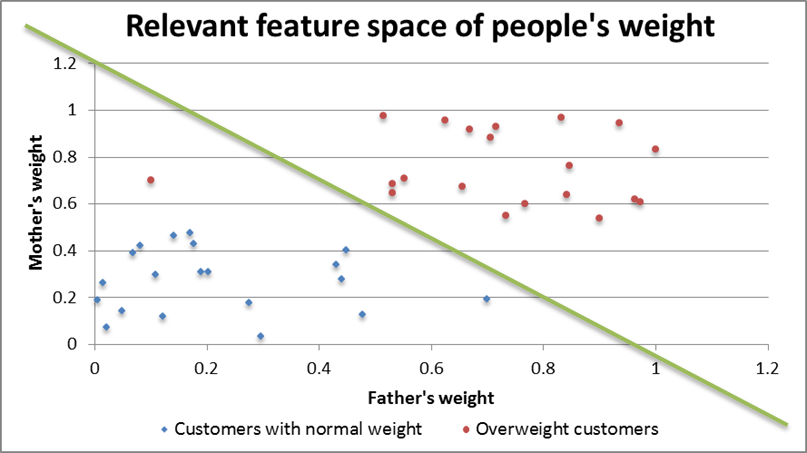
\includegraphics[width=0.8\textwidth]{../Images/example02}        
	\caption{Relevant variables helps to build better predictor models.}
	\label{fig:example01}
\end{figure}
\end{Example}
\end{frame}

\begin{frame}
\frametitle{Problem and Motivation}
\begin{itemize}
	\item Some FSS techniques (Filters) assume variables are independent and are very popular because of low computational cost.
	\item Real world behaves different because variables may influence others but this interaction is usually hidden i.e. in Bioinformatics.
	\item Prediction accuracy could be affected if dependencies are ignored.
	\item Multivariate FSS methods search for feature subsets and possible dependency relationships between them.
	\item The challenge is then to design novel feature selection methods that take advantage of multivariate power combined with high-accuracy classifiers, such as kernel classifiers, to obtain improved prediction and explanatory performance.
\end{itemize}
\end{frame}
\begin{frame}
\frametitle{Research Hypothesis}
\pause
\begin{center}
Given a set of observations taken from a particular phenomenon where dependencies among variables exist but are hidden, the selection of a subset of relevant variables is \emph{feasible} with a method that combines iterative estimation of dependency networks coupled with weighted-kernel classifiers, in such a way the method will provide a predictor model that \emph{improves} the understanding of the problem domain when compared with other techniques based on independence assumptions.
\end{center}
\end{frame}